%!TEX root = ttc14-fixml.tex

\section{Meta-Models}
\label{sec:AppendixMetaModels}

%\enlargethispage{20mm}

\subsection{XML Meta-Model}

The XML model specified in the case study description~\cite{Lano2014}.

\begin{figure}[h!bt]
  \centering
  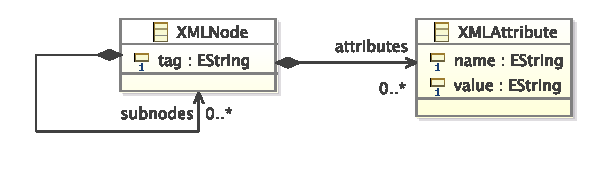
\includegraphics[width=.6\textwidth]{figures/XMLMetaModel.pdf}
  \caption{XML meta-model}
  \label{fig:AppendixXMLMetaModel}
\end{figure}

\subsection{ObjLang Meta-Model}

The meta-model representing an object oriented language originating from the Featherweight Java model~\cite{Igarashi2001} (concretely from the version available at the EMFtext website\footnote{\url{http://www.emftext.org/index.php/EMFText_Concrete_Syntax_Zoo_Featherweight_Java}}).

\begin{figure}[h!bt]
  \centering
  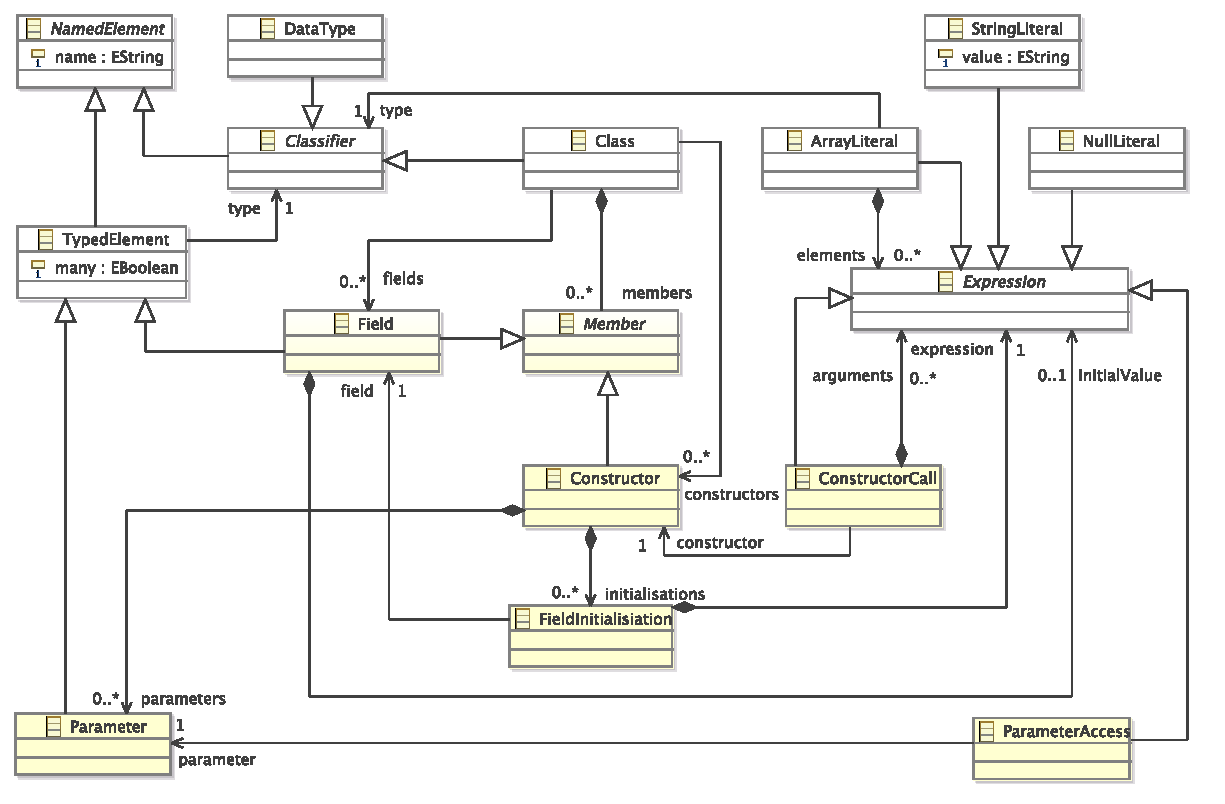
\includegraphics[width=\textwidth]{figures/ObjLangMetaModel.pdf}
  \caption{ObjLang meta-model}
  \label{fig:AppendixObjLangMetaModel}
\end{figure}


\section{XML File to XML Model Transformation}
\label{sec:AppendixXMLTransfromation}

\begin{scalacode}
protected def parseNodes(nodes: Iterable[Node]): Iterable[XMLNode] = {
  val elems = nodes collect { case e: Elem => e }

  for (elem <- elems) yield XMLNode(
    tag = elem.label,
    subnodes = parseNodes(elem.child),
    attributes = parseAttributes(elem.attributes))
}

protected def parseAttributes(metaData: MetaData) =
  metaData collect {
    case e: xml.Attribute => XMLAttribute(name = e.key, value = e.value.toString)
  }
\end{scalacode}


\section{XML Model to ObjLang Model Transformation Rules}
\label{sec:AppendixTransformationRules}

\begin{scalacode}
def ruleXMLNode2DefaultConstructor(s: XMLNode, t: Constructor) {
  s.allSameSiblings foreach (associate(_, t))
}
\end{scalacode}

\begin{scalacode}
def ruleXMLNode2NonDefaultConstructor(s: XMLNode, t: Constructor) = guardedBy {
  !s.isEmptyLeaf
} transform {

  s.allSameSiblings foreach (associate(_, t))

  for (e <- (s.allAttributes ++ s.allSubnodes.distinctBy(_.tag))) {
    val param = e.sTarget[Parameter]
    val field = e.sTarget[Field]

    t.parameters += param
    t.initialisations += FieldInitialisiation(
      field = field,
      expression = ParameterAccess(parameter = param))
  }
}
\end{scalacode}

\begin{scalacode}
def ruleXMLAttribute2ConstructorParameter(s: XMLAttribute, t: Parameter) {
  t.name = checkName(s.name)
  t.type_ = s.sTarget[Field].type_
}
\end{scalacode}

\begin{scalacode}
def ruleXMLNode2ConstructorParameter(s: XMLNode, t: Parameter) {
  val field = s.sTarget[Field]

  t.name = field.name
  t.many = field.many
  t.type_ = field.type_
}
\end{scalacode}

\begin{scalacode}
@LazyUnique
def ruleXMLAttribute2Field(s: XMLAttribute, t: Field) {
  t.name = checkName(s.name)

  t.type_ = DTString
  t.initialValue = StringLiteral(s.value)
}
\end{scalacode}

\begin{scalacode}
@LazyUnique
def ruleXMLNode2Field(s: XMLNode, t: Field) {
  val allSiblings = s.allSameSiblings
  allSiblings foreach (associate(_, t))

  t.type_ = s.sTarget[Class]

  val groups = (s +: allSiblings) groupBy (_.eContainer)
  val max = groups.values map (_.size) max

  if (max > 1) {
    t.name = s.tag + "_objects"
    t.many = true
    val init = ArrayLiteral(type_ = s.sTarget[Class])
    val siblings = groups(s.eContainer)
    
    init.elements ++= siblings.sTarget[ConstructorCall]
    init.elements ++= 0 until (max - siblings.size) map (_ => NullLiteral())
    t.initialValue = init
  } else {
    t.name = s.tag + "_object"
    t.initialValue = s.sTarget[ConstructorCall]
  }
}  
\end{scalacode}

\begin{scalacode}
@Lazy
def ruleXMLNode2ConstructorCall(s: XMLNode, t: ConstructorCall) {
  val constructor = s.sTargets[Constructor]
    .find { c =>
      (c.parameters.isEmpty && s.isEmptyLeaf) ||
      (c.parameters.nonEmpty && !s.isEmptyLeaf)
    }
    .get

  t.constructor = constructor

  t.arguments ++= {
    for {
      param <- constructor.parameters
      source = param.sSource.get
    } yield {
      source match {
        case attr: XMLAttribute =>
          // we can cast since attributes have always primitive types
          val dataType = param.type_.asInstanceOf[DataType]

          s.attributes
            .find(_.name == attr.name)
            .map { local => StringLiteral(local.value) }
            .getOrElse(NullLiteral())

        case node: XMLNode =>
          s.subnodes.filter(_.tag == node.tag) match {

            case Seq() if !param.many =>
              NullLiteral()
            case Seq(x) if !param.many =>
              x.sTarget[ConstructorCall]
            case Seq(xs @ _*) =>
              val groups = (node +: node.allSameSiblings) groupBy (_.eContainer)
              val max = groups.values map (_.size) max
              
              val init = ArrayLiteral(type_ = param.type_)
              init.elements ++= xs.sTarget[ConstructorCall]
              init.elements ++= 0 until (max - xs.size) map (_ => NullLiteral())
              init
          }
      }
    }
  }
}
\end{scalacode}

\section{Handling Constructor Arguments}
\label{sec:AppendixConstructorArguments}

The number of same-tag sibling nodes can vary within a parent node.
For example:

\inputminted[fontsize=\fontsize{8}{8},linenos,numbersep=5pt,frame=lines,framesep=2mm]{xml}{listings/variable-siblings.xml}

The \Scala|Sub| should be represented by an array field and the default initialization of \Scala|PosRpt| should equal to the following (in Java):
%
\begin{javacode}
public Pty[] Pty_objects = new Pty[] { 
  new Pty("OCC", "21", null, new Sub[] { null, null }),
  new Pty("C", "38", null, new Sub[] { new Sub("ZZZ", "2", null), null }),
  new Pty("C", "38", "Q", new Sub[] { new Sub("ZZZ", "2", null), new Sub("ZZZ", "3", "X") }) 
};
\end{javacode}
%
Note that the first and second instances of \Scala|Pty| contain two and one \Scala|null| respectively in the place of missing \Scala|Sub| subnode.

The \Scala|ConstructorCall| used for field initializations in the \Scala|ruleXMLNode2Field| is created from an XML node using the last rule in the transformation:
%
\begin{scalacode}
@Lazy
def ruleXMLNode2ConstructorCall(s: XMLNode, t: ConstructorCall) {
  val constructor = s.sTargets[Constructor]
    .find { c =>
      (c.parameters.isEmpty && s.isEmptyLeaf) ||
      (c.parameters.nonEmpty && !s.isEmptyLeaf)
    }
    .get

  t.constructor = constructor

  t.arguments ++= {
    for {
      param <- constructor.parameters
      source = param.sSource.get
    } yield {
      source match {
        case attr: XMLAttribute =>
          // we can cast since attributes have always primitive types
          val dataType = param.type_.asInstanceOf[DataType]

          s.attributes
            .find(_.name == attr.name)
            .map { local => StringLiteral(local.value) }
            .getOrElse(NullLiteral())

        case node: XMLNode =>
          s.subnodes.filter(_.tag == node.tag) match {

            case Seq() if !param.many =>
              NullLiteral()
            case Seq(x) if !param.many =>
              x.sTarget[ConstructorCall]
            case Seq(xs @ _*) =>
              val groups = (node +: node.allSameSiblings) groupBy (_.eContainer)
              val max = groups.values map (_.size) max
              
              val init = ArrayLiteral(type_ = param.type_)
              init.elements ++= xs.sTarget[ConstructorCall]
              init.elements ++= 0 until (max - xs.size) map (_ => NullLiteral())
              init
          }
      }
    }
  }
}
\end{scalacode}  

First we need to find which constructor shall be used depending on whether the given XML node (or any of its same-tag siblings) contains any attributes or subnodes.
Next, we need to resolve the arguments for the case of non-default constructor.
We do this by using the sources, \Ie, the source elements (XML node or XML attribute) that were used to create the constructor parameters.
\SIGMA provides \Scala|sSource| method that is the inverse of \Scala|sTarget| call with the difference that it will not trigger any rule execution.
In the pattern matching we need to cover all possible cases such as an attribute defined locally or an attribute defined in a same-tag sibling, thus using \Scala|null| for its initialization.


\section{M2T Transformation Class Hierarchy}
\label{sec:AppendixM2TClassHierarchy}

\begin{figure}[h!bt]
  \centering
  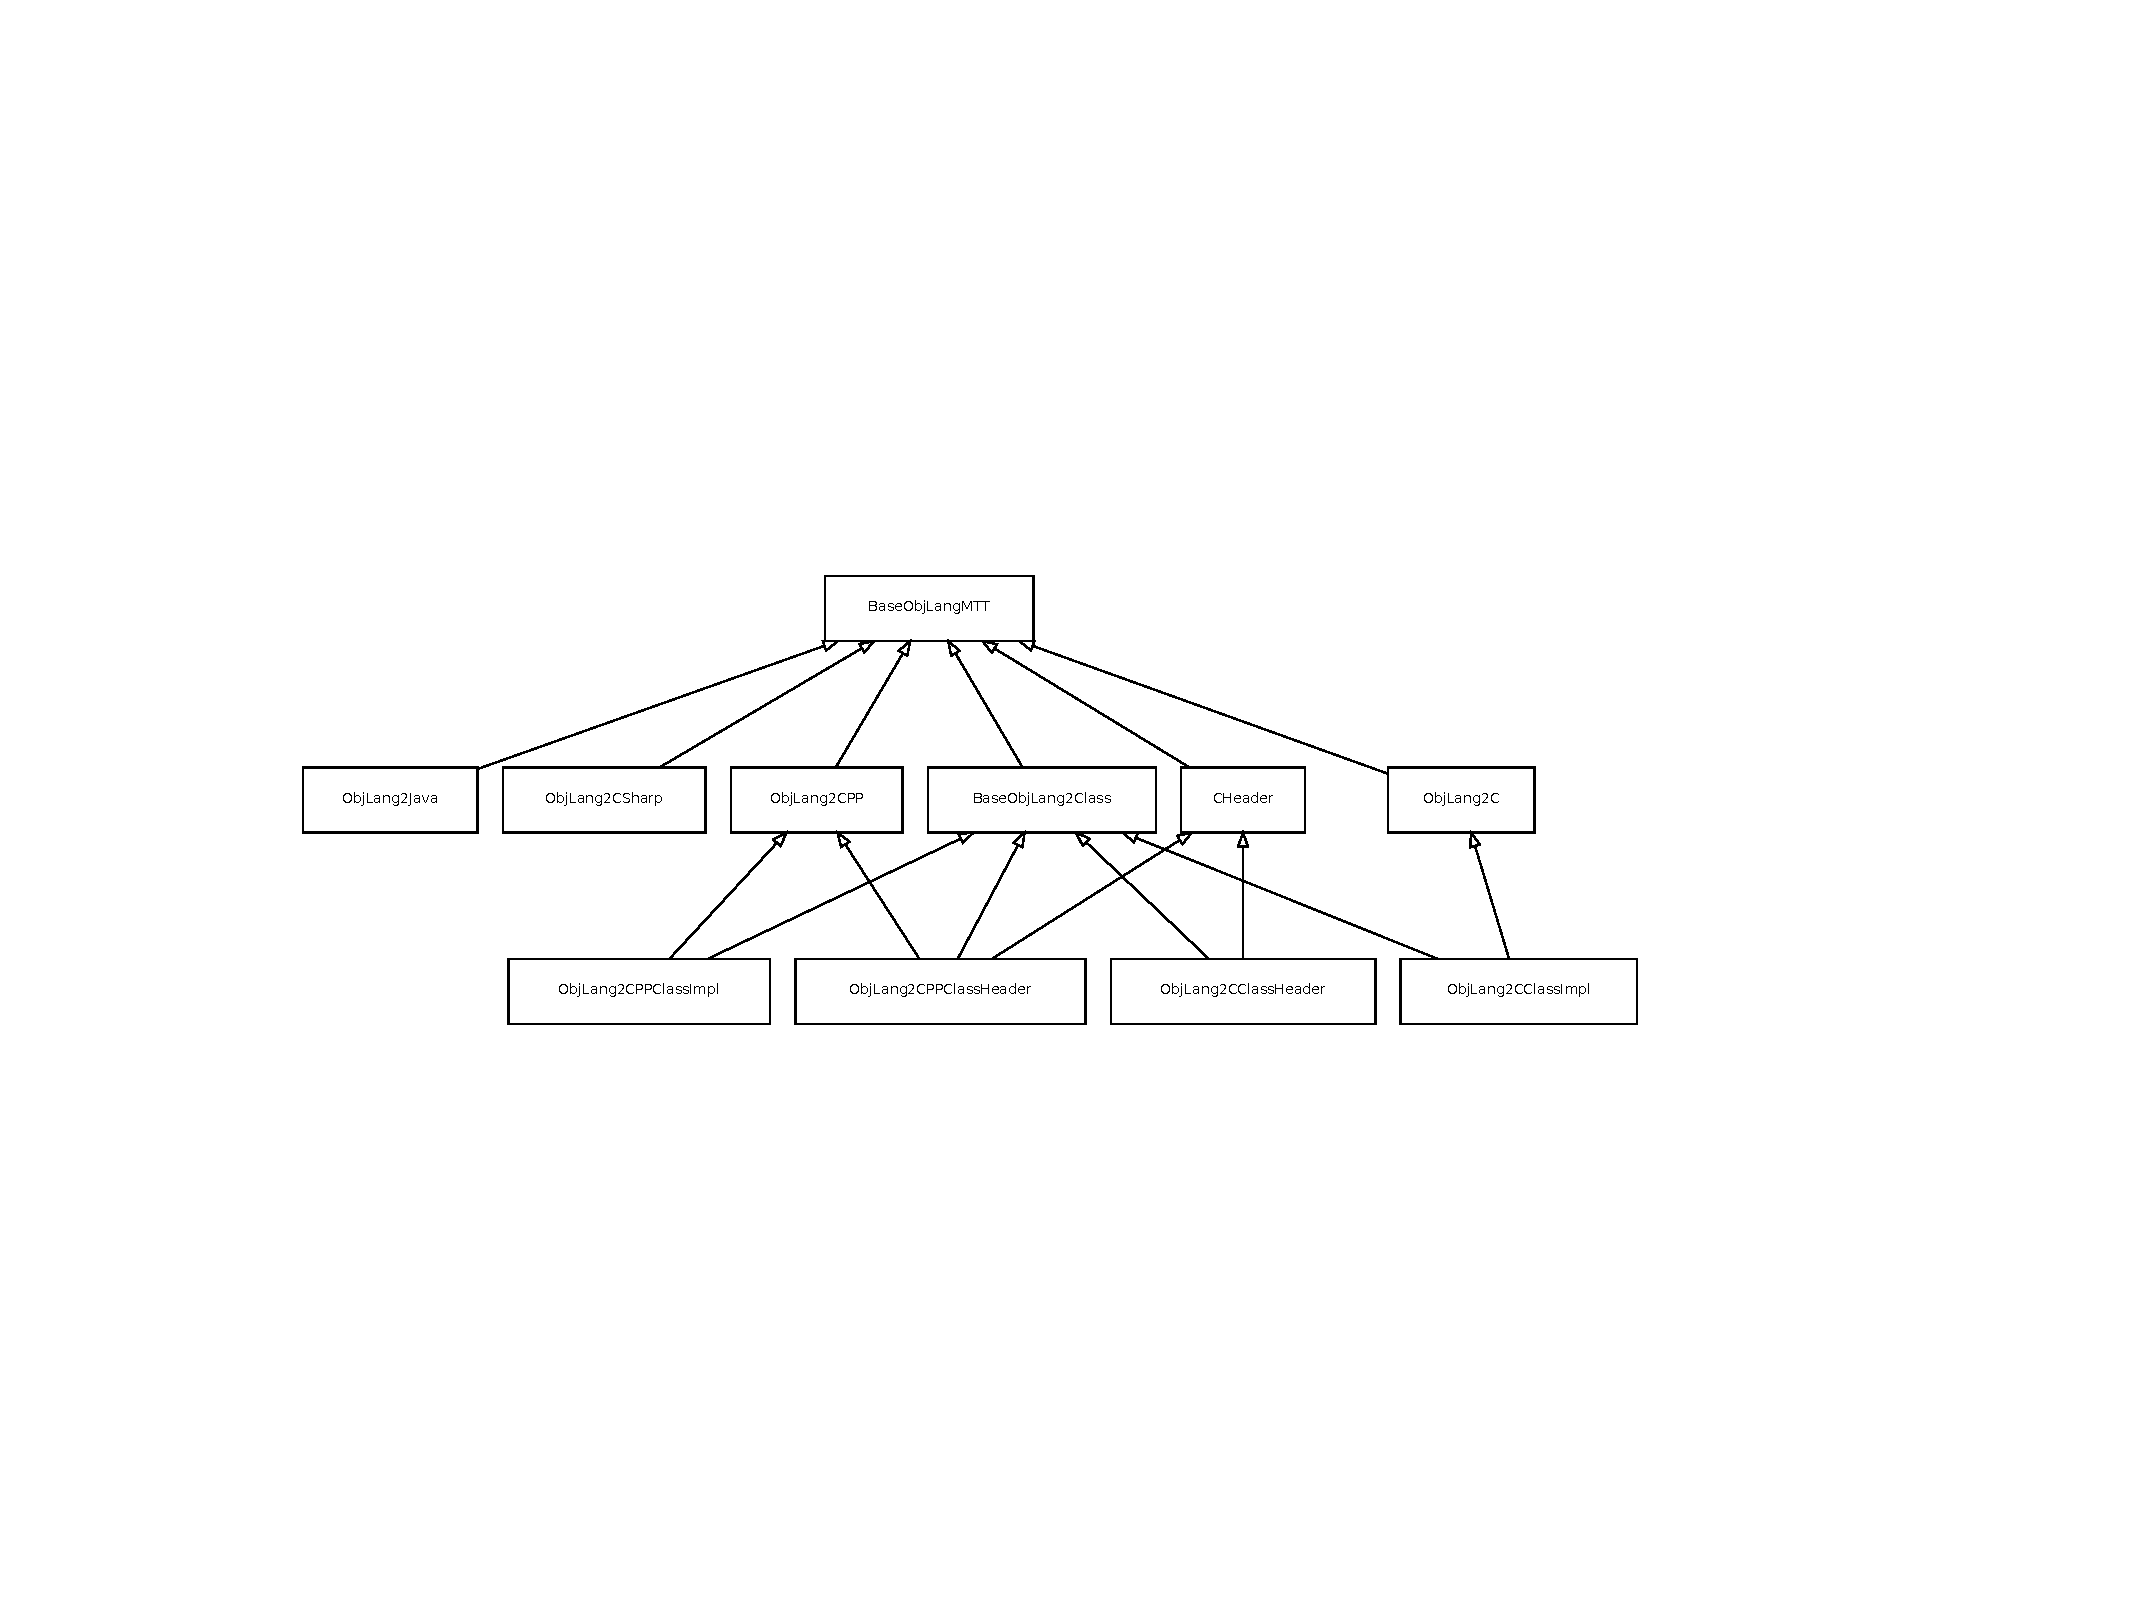
\includegraphics[width=\textwidth]{figures/M2TClassHierarchy.pdf}
  \caption{M2T transformation class hierarchy including C code generation}
  \label{fig:AppendixM2TClassHierarchy}
\end{figure}

\begin{table}[h!]
	\centering
  \begin{tabular}{l|l}
  \hline
  \textbf{File name}                  & \textbf{Source line of code} \\ \hline
  ObjLang2C.scala              & 50                  \\
  ObjLang2CClassImpl.scala     & 42                  \\
  ObjLang2CPPClassHeader.scala & 38                  \\
  BaseObjLangMTT.scala         & 35                  \\
  ObjLang2CClassHeader.scala   & 35                  \\
  BaseObjLang2Class.scala      & 33                  \\
  ObjLang2CPP.scala            & 27                  \\
  ObjLang2CPPClassImpl.scala   & 26                  \\
  ObjLang2Java.scala           & 15                  \\
  ObjLang2CSharp.scala         & 15                  \\
  CHeader.scala                & 15                  \\ \hline
  \textbf{Total}                        & \textbf{331}                 \\ \hline
  \end{tabular}
  \caption{Source lines of code for the complete M2T transformation including C code generation}
\end{table}


\section{Data Type Heuristics}
\label{sec:AppendixGuessDataType}

\begin{scalacode}
  // basic types
  val DTString = DataType(name = "string")
  val DTDouble = DataType(name = "double")
  val DTLong = DataType(name = "long")
  val DTInteger = DataType(name = "int")

  // it also stores the promotion ordering from right to left
  val Builtins = Seq(DTString, DTDouble, DTLong, DTInteger)

  private val PDouble = """([+-]?\d+.\d+)""".r
  private val PInteger = """([+-]?\d+)""".r

  def guessDataType(value: String): DataType = value match {
    case PDouble(_) => DTDouble
    case PInteger(_) => Try(Integer.parseInt(value)) map (_ => DTInteger) getOrElse (DTLong)
    case _ => DTString
  }

  def guessDataType(values: Seq[String]): DataType =
    values map guessDataType reduce { (a, b) =>
      if (Builtins.indexOf(a) < Builtins.indexOf(b)) a else b
    }
\end{scalacode}


\section{Generating C Code}
\label{sec:AppendixGeneratingCCode}

Input document:

\inputminted[fontsize=\fontsize{8}{8},linenos,numbersep=5pt,frame=lines,framesep=2mm]{xml}{listings/example-for-c-code.xml}

\noindent Generated C code:

\begin{ccode}
#ifndef _Pty_H_
#define _Pty_H_

#include <stdlib.h>

#include "Sub.h"

typedef struct {
  char* _R;
  char* _ID;
  Sub** Sub_objects;
} Pty;

Pty* Pty_new();
Pty* Pty_init_custom(Pty* this, char* _R, char* _ID, Sub** Sub_objects);
Pty* Pty_init(Pty* this);

#endif // _Pty_H_	
\end{ccode}
%
\begin{ccode}
#include "arrays.h"

#include "Pty.h"

Pty* Pty_new() {
  return (Pty*) malloc(sizeof(Pty));
}

Pty* Pty_init_custom(Pty* this, char* _R, char* _ID, Sub** Sub_objects) {
  this->_R = _R;
  this->_ID = _ID;
  this->Sub_objects = Sub_objects;
  return this;
}

Pty* Pty_init(Pty* this) {
  this->_R = "21";
  this->_ID = "OCC";
  this->Sub_objects = (Sub**) new_array(2, Sub_init_custom(Sub_new(), "2", "ZZZ"), NULL);
  return this;
}
\end{ccode}

\section{Execution Times of the Core Problem Solution}
\label{sec:AppendixExecutionTime}

\begin{table}[h!]
  \centering
  \begin{tabular}{ l | r | r | r | r }
    \hline
    \textbf{Message} & \textbf{T2M} & \textbf{M2M} & \textbf{M2T} & \textbf{Total} \\
    \hline
    \texttt{test1}   & 9      & 70     & 191   & 270  \\
    \texttt{test2}   & 27     & 351    & 284   & 662  \\
    \texttt{test5}   & 1201   & 2734   & 459   & 4394 \\
    \texttt{test6}   & 376    & 1387   & 393   & 2156 \\
    \hline
    \textbf{Total}   & 1613   & 4542   & 1327  & 7482 \\
    \hline
  \end{tabular}
  \caption{Execution times for the test \FIXML messages as measured on SHARE (in milliseconds)}
  \label{tab:ExecutionTime}
\end{table}

